\documentclass[10pt,twocolumn]{article}

\usepackage[T1]{fontenc}
\usepackage[utf8]{inputenc}
\usepackage[margin=0.75in]{geometry}
\usepackage{amsmath,amssymb,amsfonts}
\usepackage{graphicx}
\usepackage{caption}
\usepackage{booktabs}
\usepackage{balance}
\usepackage{abstract}
\usepackage{microtype}
\usepackage{times}
\usepackage[hidelinks]{hyperref}
\usepackage{enumitem}
\setlist{nosep,leftmargin=1.4em}
\makeatletter
\setlength{\@fptop}{0pt}
\setlength{\@dblfptop}{0pt}
\makeatother

\title{\vspace{-2.5em}\textbf{Sovereign Cognitive Digital Twins: Fusing 6G ISAC,
AI-RAN, and Zero-Trust Edge Grids for Climatic Resilience in
Archipelagic and Island Nations}}

\author{
Zoe Aiyanna M. Cayetano\thanks{zoe@amini} \quad George M. Gichuru\thanks{george@amini}\\
\small Amini Labs, Nairobi, Kenya \\[0.3em]
\small \textit{Working draft --- \today}}
\date{}

\begin{document}
\twocolumn[
\maketitle
\begin{onecolabstract}
\noindent\textbf{Abstract}---Climate-hazard-prone archipelagic and small-island
developing states (SIDS) confront an existential risk profile---accelerating
sea-level rise, intensifying tropical cyclones, and storm surge---while
simultaneously suffering the sparse ground-based instrumentation that makes
timely hazard perception difficult. This paper argues for a paradigm shift from
passive cellular connectivity to the \emph{Network as a Sensor} (NaaS), realized
through a \emph{Sovereign Cognitive Digital Twin} (S-CDT): a federated national
digital twin whose perceptual substrate is the 6G radio interface itself. Rather
than deploying expensive, disjoint environmental sensing systems, a vulnerable
nation can reuse the Integrated Sensing and Communication (ISAC) waveforms of its
own network as a distributed radar mesh, feeding a closed-loop cognitive
orchestration engine for real-time state estimation, predictive hazard
forecasting, and automated mitigation. We ground the architecture in the UK
National Digital Twin Programme's federation lesson and the Gemini Principles;
we specify a six-layer S-CDT stack in which ISAC structurally collapses the
boundary between the dynamic-data and communication layers; we map the physical
layer to the ETSI GR ISC~001 and 3GPP Release~19 sensing frameworks; and we
formulate a belief-state control loop---an Extended Kalman Filter feeding a
Proximal Policy Optimization agent---that remains stable under O-RAN telemetry
delay. Finally, we treat data sovereignty and physical-layer zero-trust security
as first-order design constraints, proposing subsystem disaggregation,
cross-layer anomaly detection, and privacy-tiered waveforms. Barbados
($166~\mathrm{km}^2$, $\sim$280k population) is used as a tractable reference
deployment, with the Philippines as an archipelagic generalization.

\vspace{0.5em}
\noindent\textbf{Index Terms}---digital twin, 6G, integrated sensing and
communication (ISAC), AI-RAN, climate resilience, small island developing
states, zero-trust, data sovereignty.
\vspace{1.5em}
\end{onecolabstract}
]

\section{Introduction}

\subsection{The Climate Existential Threat}
Archipelagic and small-island developing states occupy the sharp edge of
anthropogenic climate change. For nations such as Barbados in the Caribbean and
the Philippines in the western Pacific, sea-level rise, coastal erosion, and the
intensification of typhoons and storm surge are not distant projections but
present-tense determinants of national survival, economic continuity, and
population safety~\cite{undp_sids,wef_barbados}. These same nations are, in
general, the most weakly instrumented: dense networks of tide gauges, weather
radar, and hydrological sensors are capital-intensive to deploy and, critically,
fragile precisely during the extreme events for which they are most needed.
The result is a perception gap---decisions with hours-to-minutes stakes made on
data with hours-to-days latency.

\subsection{A Paradigm Shift: The Network as a Sensor}
We propose closing that gap not by multiplying dedicated sensors but by
re-conceiving infrastructure the nation is already motivated to build. The
transition from fifth- to sixth-generation mobile networks introduces
\emph{Integrated Sensing and Communication} (ISAC), in which the radio interface
that carries data simultaneously performs radar-like sensing of its
environment~\cite{ericsson_isac,etsi_isc001}. Under this \emph{Network as a
Sensor} (NaaS) paradigm, every base station is also an environmental
instrument, and the coverage footprint of the network becomes the sensing
footprint of the nation.

\subsection{Thesis and Contributions}
Our thesis is that vulnerable nations can deploy a unified \emph{Sovereign
Cognitive Digital Twin} (S-CDT) that uses the 6G radio interface as a
continuous perceptual nervous system, providing real-time modeling, predictive
hazard forecasting, and closed-loop disaster mitigation, under national
sovereign control of models and data. This paper contributes: (i) a federated
S-CDT reference architecture aligned with established national-digital-twin
governance (\S\ref{sec:baseline}); (ii) a six-layer stack in which ISAC
collapses the dynamic-data and communication layers (\S\ref{sec:stack}); (iii)
a standards-grounded treatment of the physical sensing layer
(\S\ref{sec:physical}); (iv) a belief-state cognitive-orchestration loop robust
to RAN telemetry delay (\S\ref{sec:cognitive}); and (v) a sovereign,
physical-layer zero-trust security and privacy design (\S\ref{sec:security}).

\section{Grounding the Baseline: The National Digital Twin Paradigm}
\label{sec:baseline}

\subsection{The Federated Architecture}
The single most consequential design decision is to reject the monolith. The UK
National Digital Twin Programme's central, hard-won lesson is that a national
twin is not one model of everything but a \emph{federated ecosystem} of
domain-specific twins, connected through shared identifiers, open standards, and
a common trust framework~\cite{ndtp,gemini}. Federation is what makes the system
buildable incrementally, governable across institutional owners, and resilient
to the failure or replacement of any single component.

\subsection{Governance via the Gemini Principles}
We structure S-CDT governance around the nine Gemini
Principles~\cite{gemini}, grouped as:
\begin{itemize}
\item \textbf{Purpose}---public good, actionable insight, and measurable
economic and climatic value.
\item \textbf{Trust}---security by default (here elevated to \emph{zero trust}),
transparent data provenance, and high-quality validation.
\item \textbf{Function}---federated interoperability, scalability, and long-term
evolutionary capability.
\end{itemize}
For a sovereign deployment the ``trust'' cluster is load-bearing: the twin's
outputs must be defensible enough to justify evacuations and to underwrite
climate finance, which demands auditable provenance rather than best-effort
data hygiene.

\subsection{The Design Brackets}
Two operational national/urban twins bracket the design space. The
\emph{built-environment bracket} is Virtual Singapore (Dassault Syst\`emes with
GovTech, SLA, and NRF): a semantically rich 3D model fused with live smart-nation
sensor feeds, driving micro-mobility, solar-potential, and flood
simulation~\cite{vsg}. The \emph{earth-system bracket} is Destination Earth
(DestinE) of the European Commission, with ESA, EUMETSAT, and ECMWF: planetary
climate-adaptation and extreme-events twins running on high-performance-computing
architectures over a multi-source data lake~\cite{destine}. The S-CDT merges the
brackets---island-scale built-environment fidelity coupled to earth-system
climate dynamics---and adds the 6G shift that neither exemplar yet exploits:
\emph{the connecting network is itself the primary real-time sensor}, redefining
the boundary of ``live data.''

\section{The Unified S-CDT Layered Stack and the ISAC Transformation}
\label{sec:stack}

\subsection{The Core Stack}
The S-CDT is organized as six layers over a vertical trust-and-governance spine:

\begin{enumerate}
\item \textbf{Geospatial Ground Truth}---high-resolution terrain, bathymetry,
building envelopes, and critical utility networks. Barbados's
$166~\mathrm{km}^2$ area and $\sim$280k population make complete, high-fidelity
national modeling extraordinarily tractable relative to a large state.
\item \textbf{Systems of Record}---dynamic registries of land, business,
population, and infrastructure assets.
\item \textbf{Dynamic Data / Nervous System}---fusion of satellite Earth
Observation, IoT telemetry, and the 6G ISAC radio-sensing network.
\item \textbf{Simulation and Surrogates}---physics-based hydrology and coastal
hydrodynamic models, statistical agent-based evacuation models, and deep-learning
surrogate models for real-time ray-tracing and wave propagation.
\item \textbf{Synchronization Engine}---reconstruction of current-time state
estimates from dynamic physical telemetry.
\item \textbf{Interaction and Orchestration}---generative-AI natural-language
query interfaces, executive dashboards, and automated control-API pipelines.
\end{enumerate}

\subsection{The ISAC Structural Fusion}
In the classical layered view, the communication infrastructure is plumbing that
\emph{transports} data produced by a physically separate sensing layer. ISAC
dissolves this separation: the physical radio waves of the network double as a
distributed radar mesh, so the Dynamic-Data Layer and the communication
infrastructure become one substrate~\cite{ericsson_isc001,etsi_isc001}. Sensor
deployment as a distinct capital programme becomes largely obsolete; instead,
sensing is a software-and-spectrum function of the network the nation deploys
for connectivity. For an operator-integrator this collapses three roles into a
single asset---the network is simultaneously (a)~physical infrastructure the twin
\emph{models}, (b)~the backbone that \emph{carries} twin data, and (c)~the
distributed sensor that \emph{feeds} the twin.

\section{The Network as the Perceptive Nervous System: Physical Layer and Standards}
\label{sec:physical}

\subsection{Dual-Function Radar-Communication}
At the physical layer, ISAC is realized as Dual-Function Radar-Communication
(DFRC): a 6G base station uses shared spectrum and shared hardware to transmit a
waveform that simultaneously delivers high-throughput data and yields
radar-grade observables---range, angle (angle-of-arrival), radial velocity
(Doppler), and micro-structure---by processing echoes and multipath. The ISAC
propagation channel is conveniently decomposed as
\begin{equation}
\mathbf{H}_{\mathrm{ISAC}} = \mathbf{H}_{\mathrm{target}} +
\mathbf{H}_{\mathrm{background}},
\end{equation}
where $\mathbf{H}_{\mathrm{target}}$ captures returns from dynamic sensing
targets and $\mathbf{H}_{\mathrm{background}}$ models the quasi-static
environment~\cite{tr38901,rel19survey}. Estimating and subtracting a learned
background is precisely what lets the network isolate a moving hazard---or a
weather cell---from clutter.

\subsection{Standardization Milestones}
\textbf{ETSI.} The ETSI ISG ISAC group's first report, GR ISC~001 (April 2025),
establishes 18 advanced use cases, three integration levels (tight,
intermediate, and loose), and six sensing modes for 6G
sensing~\cite{etsi_isc001}; subsequent reports (e.g.\ GR ISC~003, 2026) address
system and RAN architectures~\cite{etsi_isc003}. \emph{(We note a common
mis-citation: the 18-use-case report is GR ISC~001, not GR ISC~004.)}

\noindent\textbf{3GPP.} Release~19 (study concluded May 2025) specifies wireless
sensing use cases in TR~22.837 and extends the TR~38.901 channel model for
ISAC~\cite{tr22837,tr38901}. Six sensing modes are defined by
transmitter/receiver placement:
\begin{itemize}
\item \textbf{Monostatic}: TRP-based (Tx/Rx co-located at a
transmission-reception point) and UE-based.
\item \textbf{Bistatic}: TRP$\rightarrow$TRP, TRP$\rightarrow$UE,
UE$\rightarrow$TRP, and UE$\rightarrow$UE.
\end{itemize}
Sensing spans FR1, the emerging FR3 mid-band, and FR2 mmWave, trading coverage
against range/velocity resolution. Release~20 continues the architecture study.

\subsection{Climbing the Sensing Maturity Ladder}
Each environmental sub-twin climbs the maturity ladder
independently---\emph{Descriptive} $\rightarrow$ \emph{Diagnostic} $\rightarrow$
\emph{Predictive} $\rightarrow$ \emph{Prescriptive} $\rightarrow$
\emph{Autonomous}---with the predictive-and-above rungs driven natively by edge
AI and network sensing. Three exemplar capabilities:

\paragraph{Moving-object detection.} Coordinated, multi-static tracking of
non-cooperative aerial hazards (unregistered drones over critical
infrastructure) and prioritization of emergency vehicles, using Doppler
signatures without requiring the target to carry a device.

\paragraph{Environmental and weather mapping.} Hyper-local rainfall estimation
inferred from frequency-specific attenuation. Specific attenuation follows the
ITU-R power law
\begin{equation}
\gamma_R = k\,R^{\alpha} \quad [\mathrm{dB/km}],
\end{equation}
with rain rate $R$ and band-dependent coefficients $k,\alpha$~\cite{itur838};
the path integral of $\gamma_R$ is observable as excess attenuation in the
channel state, so mmWave/FR3 links act as a dense mesh of virtual rain
gauges~\cite{raingauge}, enabling flash-flood and track-washout prediction well
below the resolution of sparse ground radar.

\paragraph{Radio-environment analysis.} Continuous RF fingerprinting and
multipath-delay-profile indexing dynamically update the local clutter map that
constitutes $\mathbf{H}_{\mathrm{background}}$, both improving sensing and
providing a change-detection channel in its own right.

\section{Closed-Loop Cognitive Orchestration: AI-RAN and Belief-State Control}
\label{sec:cognitive}

\subsection{AI-RAN Convergence}
Perception without timely action is merely telemetry. We distribute intelligence
into the Radio Access Network itself: model training via federated learning
across sites (keeping raw observations local), and inference at the O-RAN
Near-Real-Time and Non-Real-Time RAN Intelligent Controllers
(RICs)~\cite{oran_isac}. The Non-RT RIC hosts the digital-twin models and policy
learning; the Near-RT RIC executes low-latency control (beam and resource
allocation) as an xApp.

\subsection{Belief-State Control under Telemetry Delay}
The central control obstacle is delay: O-RAN telemetry can reach the controller
tens of milliseconds late (up to $\sim$100~ms), so the instantaneous
measurement is a stale view of a fast-moving hazard field. We therefore control
on a \emph{belief state} rather than raw observations. An Extended Kalman Filter
(EKF) running inside the twin maintains an estimate of the latent environmental
and network state $\mathbf{x}_t$. The prediction step is
\begin{align}
\hat{\mathbf{x}}_{t|t-1} &= f(\hat{\mathbf{x}}_{t-1|t-1},\mathbf{u}_t),\\
\mathbf{P}_{t|t-1} &= \mathbf{F}_t \mathbf{P}_{t-1|t-1}\mathbf{F}_t^{\top} +
\mathbf{Q}_t,
\end{align}
with $\mathbf{F}_t = \left.\partial f/\partial\mathbf{x}
\right|_{\hat{\mathbf{x}}_{t-1|t-1}}$. To absorb a measurement delay $\tau$, the
update fuses the delayed observation $\mathbf{z}_{t-\tau}$ against the
correspondingly retrodicted state,
\begin{align}
\mathbf{K}_t &= \mathbf{P}_{t|t-1}\mathbf{H}_t^{\top}
\!\left(\mathbf{H}_t \mathbf{P}_{t|t-1}\mathbf{H}_t^{\top}
+ \mathbf{R}_t\right)^{-1},\\
\hat{\mathbf{x}}_{t|t} &= \hat{\mathbf{x}}_{t|t-1}
+ \mathbf{K}_t\!\left(\mathbf{z}_{t-\tau}
- h(\hat{\mathbf{x}}_{t-\tau|t-1})\right).
\end{align}
The resulting belief $s_t = (\hat{\mathbf{x}}_{t|t}, \mathbf{P}_{t|t})$---the
mean estimate together with its covariance---is a sufficient statistic that
explicitly carries the controller's uncertainty into the decision.

\subsection{Reinforcement-Learned Orchestration}
A Proximal Policy Optimization (PPO) agent maps the belief state to control
actions $a_t$---beamforming power, sensing dwell/scan allocation, and mode
selection across the six ISAC modes---maximizing the clipped surrogate
objective
\begin{equation}
L^{\mathrm{CLIP}}(\theta) = \mathbb{E}_t\!\left[\min\!\big(\rho_t(\theta)\hat{A}_t,\;
\mathrm{clip}(\rho_t(\theta),1-\epsilon,1+\epsilon)\hat{A}_t\big)\right],
\end{equation}
with probability ratio $\rho_t(\theta)=\pi_\theta(a_t\mid s_t)/
\pi_{\theta_{\mathrm{old}}}(a_t\mid s_t)$ and advantage estimate $\hat{A}_t$. The
reward balances the competing objectives of a shared sensing/communication
resource,
\begin{equation}
r_t = \alpha\,\mathcal{A}_{\mathrm{sens}}
+ \beta\,\mathcal{T}_{\mathrm{comm}}
- \gamma\,\mathcal{E}
- \delta\,\mathcal{R}_{\mathrm{sec}},
\end{equation}
rewarding sensing accuracy $\mathcal{A}_{\mathrm{sens}}$ and communication
throughput $\mathcal{T}_{\mathrm{comm}}$ while penalizing energy $\mathcal{E}$
and residual security risk $\mathcal{R}_{\mathrm{sec}}$. Under an active-hazard
regime the learned policy shifts resource toward tracking; under nominal
conditions it favors throughput.

\subsection{Edge Observation Compression}
Multi-static sensing produces high-dimensional 3D point clouds that would
saturate rate-limited emergency backhaul exactly when links are degraded. We
apply an autoencoder (AE) at the gNodeB for dimension reduction: an encoder
$f_\phi$ maps a point cloud $\mathbf{P}$ to a compact code
$\mathbf{z}=f_\phi(\mathbf{P})$, transmitted in place of the raw cloud and
reconstructed by $g_\psi$ at the core, trained to minimize
\begin{equation}
\mathcal{L}_{\mathrm{AE}} = d_{\mathrm{CD}}\!\big(\mathbf{P},
g_\psi(f_\phi(\mathbf{P}))\big) + \lambda\lVert\mathbf{z}\rVert_1,
\end{equation}
where $d_{\mathrm{CD}}$ is the Chamfer distance and the $\ell_1$ term encourages
a sparse, low-rate code. This preserves hazard-relevant geometry under a strict
backhaul budget.

\section{Sovereign Data Protection and Physical-Layer Zero Trust}
\label{sec:security}

\subsection{The Sovereign Compute Grid}
A twin that governs evacuations and underwrites climate finance is national
critical infrastructure. Climate-vulnerable nations must therefore retain
sovereign control of AI weights, models, and spatial telemetry rather than
renting perception from external cloud monopolies. The S-CDT is designed for an
on-territory sovereign compute grid---edge inference at the RAN, national core
for training and archival---so that both the raw sensing of the population and
the learned models derived from it remain under domestic jurisdiction. This is
also a resilience property: sovereign edge autonomy keeps the twin operating
when international connectivity is severed by the very disaster it must manage.

\subsection{Zero-Trust Subsystem Disaggregation}
Because the network now senses the nation, its compromise is a national-security
event, not merely a service outage. We adopt a disaggregated trust model in the
spirit of OPPO's ``Minimized Kernel~$+~N$ Subsystems'' 6G
architecture~\cite{oppo_kernel,oppo_sec}: a minimal, formally hardened kernel
provides base connectivity, while sensitive functions---national-security
sensing, emergency services, and the environmental-sensor plane---run as
isolated subsystems with independent trust domains. No plane implicitly trusts
another; the environmental-sensing plane cannot be pivoted into from a
compromised consumer-data plane.

\subsection{Cross-Layer Anomaly Detection}
Physical-layer observables are themselves a security sensor. We fuse
angle-of-arrival (AoA), Doppler shift, and channel state information (CSI) with
higher-layer protocol state to detect physical-layer attacks that are invisible
above the PHY: signal spoofing, GNSS/GPS jamming, and tampering with
Reconfigurable Intelligent Surfaces (RIS). A spoofed transmitter that is
protocol-correct but geometrically impossible (inconsistent AoA/Doppler for its
claimed identity) is flagged by the cross-layer detector.

\subsection{Privacy-by-Design Waveforms}
NaaS sensing is powerful and politically sensitive: the same channel that maps
topography can, at fine resolution, read human behavior. We organize spatial
telemetry into privacy tiers---\textbf{L1 Environmental} (terrain, hydrology,
weather), \textbf{L2 Behavioral} (aggregate mobility, presence), and \textbf{L3
Physiological} (fine micro-Doppler, e.g.\ respiration/gait)---with escalating
consent and access controls. To enforce the boundary at the physical layer we
inject calibrated noise into the reported CSI,
\begin{equation}
\tilde{\mathbf{H}} = \mathbf{H} + \mathbf{N},\qquad
\mathbf{N}\sim\mathcal{P}\big(\sigma_{\mathrm{beh}}\big),
\end{equation}
where $\mathcal{P}$ is designed to destroy the high-frequency micro-Doppler
components that carry behavioral/physiological signatures while preserving the
low-frequency structural returns needed for topography and weather sensing. The
network can thus deliver high-resolution environmental perception at L1 while
being provably unable to export L2/L3 signatures without explicit,
tier-appropriate authorization.

\section{Deployment Blueprint: Barbados and the Archipelagic Generalization}
\label{sec:deploy}

We propose a \emph{minimum viable twin} that proves the full vertical slice on a
single existential question before federating outward. Its components: (1) a
national basemap bootstrapped from Earth-observation foundation models; (2) at
least one network-derived live feed---microwave-link/CSI rainfall---designed
ISAC-ready, alongside a tide/weather feed; (3) one predictive model (coastal
inundation under a parametric storm scenario) driven by the live rainfall field;
(4) a generative natural-language query interface for decision-makers; and (5)
node and sensor attestation plus data provenance on a sovereign ledger to make
outputs finance- and evacuation-grade. Federation then proceeds domain by
domain---economy and tourism next, coupled to the climate twin through
network-derived mobility---while every newly deployed base station is specified
ISAC-ready so the sensing mesh densifies as a byproduct of connectivity
roll-out. Barbados serves as a bounded, high-fidelity reference; the Philippines
generalizes the design to a multi-thousand-island archipelago where inter-island
non-terrestrial (satellite) ISAC and edge autonomy become decisive.

\begin{figure*}[t]
\centering
\includegraphics[width=0.72\textwidth]{scdt_architecture_amini.png}
\caption{The S-CDT reference architecture referenced throughout this paper: a
six-layer stack over a vertical zero-trust and integrity spine. Sensing
(Network-as-a-Sensor) feeds the GeoPackage engine that produces spatio-temporal
data cubes; cubes are sharded across the Amini node network and anchored on Amini
Chain (content hashing, provenance, node attestation); a zero-trust integrity gate
admits only verified cubes to the national sovereign data lake that powers the
cognitive twin; orchestration closes the loop back to the sensing layer.}
\label{fig:arch}
\end{figure*}

\section{Implementation: the Barbados Digital Twin as built}
\label{sec:impl}
The preceding sections describe the target S-CDT. This section reports what has
actually been built to date on the Barbados deployment, inside the Ulap SCOPE
application, and separates shipped capability (\textbf{[B]uilt}) from
designed-but-not-yet-enforced capability (\textbf{[D]esign}) so the architecture is
not over-claimed. Measured against the sensing-maturity ladder of
\S\ref{sec:physical}, the deployed twin sits at the \emph{descriptive/diagnostic}
rungs: it renders the nation and its exposure and joins hazard return-periods to
assets, but does not yet run the predictive-and-above cognitive loop.
Figures~\ref{fig:rf-coverage}--\ref{fig:island-overview} provide compact visual
evidence of the implemented planning, provenance, inspection, interaction, and
multi-source fusion workflows.

\subsection{Mapping the deployment to the reference stack}
Figure~\ref{fig:arch} is the reference architecture; Table~\ref{tab:map} maps each
of its layers to the deployed system. The build faithfully realizes the
\emph{perceptual and serving} substrate --- layers~1, 2, 4 (catalog) and 6
(dashboards) --- while the \emph{cognitive} (5), \emph{ledgered-trust} (3) and
\emph{enforced-governance} (spine) elements remain specified and scheduled
(\S\ref{sec:roadmap}).

\begin{table*}[t]\footnotesize\centering
\caption{Reference-stack layers mapped to the Ulap SCOPE deployment.
[B]~=~built, [D]~=~design.}\label{tab:map}
\begin{tabular}{@{}p{2.5cm}p{11.1cm}p{2.0cm}@{}}
\toprule
S-CDT layer & Deployed in Ulap SCOPE today & State\\
\midrule
1. Sensing (NaaS) & Live connectors: 3D-PAWS/CHORDS weather, OpenSky flights, CelesTrak TLEs, Sentinel-2/Copernicus EO, Open-Meteo, OpenCellID. ISAC radar-sensing is not yet a feed. & [B] conv.\ sensing; [D] ISAC\\
2. GeoPackage transform & \texttt{twin\_ingest}: shapefiles $\rightarrow$ reproject $\rightarrow$ normalize $\rightarrow$ GeoPackage + PMTiles --- the GeoPackage engine at national scale. & [B]; [D] X/Y/Z/T cubes\\
3. Node network + chain & Per-layer source attribution + \texttt{catalog.json} manifest. No on-chain content-hashing or node attestation yet. & [D]\\
4. Sovereign data lake & \texttt{catalog.json} catalog served from a single GeoPackage on sovereign/edge storage; versioning by re-ingest. & [B] catalog; [D] versioned lake\\
5. Cognitive twin & Sionna RF simulation and climate-risk models exist as surrogates; no EKF belief-state loop or PPO orchestration yet. & [D]\\
6. Interaction & SCOPE web app: 3D map, twin KPIs, inspect panels, layer/hazard dashboards. & [B]; [D] closed-loop / GovChat\\
Zero-trust spine & Source attribution on every response + graceful-degrade contract. Tiering, attestation gate and integrity validation designed, not enforced. & [D]\\
\bottomrule
\end{tabular}
\end{table*}

\subsection{Data provenance: authoritative layers}
\label{sec:impl-provenance}
All 19 static layers derive from a single authoritative source, the Barbados
Geoportal of the Lands \& Surveys Department, received as 19 ESRI shapefiles
constituting a national infrastructure, hazard and vulnerability
database~\cite{bbdgeo}. Two facts govern every transformation. First, source
geometry is EPSG:21292 (Barbados 1938 / British West Indies Grid) and is reprojected
to EPSG:4326 for web mapping; a correctness invariant is that the building bounding
box must reproject to the whole island (verified at $[-59.650,\,13.045]$ to
$[-59.422,\,13.335]$). Second, critical-asset layers carry hazard return-period
fields (rainfall and coastal flood, landslide, seismic), which is what lets the twin
join assets to the climate-risk models. Table~\ref{tab:layers} is the ingested
inventory. The government \texttt{vulnerability\_*} grid is treated as authoritative
and supersedes the earlier census-derived parish proxy; the service degrades to the
lower-provenance proxy only when the grid is absent, and carries the source label
either way.

\begin{table*}[t]\scriptsize\centering
\caption{Ingested static layer inventory (real counts from \texttt{catalog.json}).
Source: Barbados Geoportal, Lands \& Surveys Dept.; CRS EPSG:21292~$\rightarrow$~EPSG:4326.
\texttt{track}~=~serving strategy.}\label{tab:layers}
\begin{tabular}{@{}p{3.2cm}llrl@{\hskip 10pt}p{6.6cm}@{}}
\toprule
Layer (twin name) & Geom & Count & Track & Twin role\\
\midrule
\texttt{buildings} & polygon & 130{,}248 & tiles & Island-wide 3D on terrain\\
\texttt{roads} & line & 705 & geojson & Road network\\
\texttt{bridges} & line & 25 & geojson & Bridges (hazard-annotated)\\
\texttt{ports} & polygon & 4 & geojson & Ports \& BGI airport hotspots\\
\texttt{antennas} & point & 100 & geojson & Telecom / RF twin\\
\texttt{drinking\_water\_network} & line & 17{,}802 & tiles & Potable mains\\
\texttt{water\_mains} & line & 17{,}966 & tiles & Water mains\\
\texttt{wastewater\_plants} & point & 48 & geojson & Wastewater plants\\
\texttt{desalination\_plants} & point & 5 & geojson & Desalination (critical)\\
\texttt{dams} & point & 39 & geojson & Dams\\
\texttt{reservoirs} & point & 34 & geojson & Reservoirs\\
\texttt{pumping\_stations} & point & 19 & geojson & Pumping stations\\
\texttt{communal\_wells} & point & 38 & geojson & Wells\\
\texttt{individual\_wells} & point & 40 & geojson & Wells\\
\texttt{major\_projects} & point & 111 & geojson & Capital projects\\
\texttt{vulnerability\_global} & polygon & 13{,}029 & tiles & Authoritative gov.\ vulnerability grid\\
\texttt{vulnerability\_population} & polygon & 13{,}029 & tiles & Population exposure\\
\texttt{vulnerability\_environmental} & polygon & 13{,}029 & tiles & Environmental exposure\\
\texttt{vulnerability\_equipment} & polygon & 13{,}029 & tiles & Equipment / economic exposure\\
\bottomrule
\end{tabular}
\end{table*}

\subsection{Live feeds}
Beyond the static export, typed connectors hydrate live layers, one documented
ingress per source: 3D-PAWS weather stations via CHORDS, Open-Meteo, OpenSky
flights, CelesTrak TLEs (NTN constellations), Sentinel-2 L2A and Copernicus DEM via
the CDSE STAC, ESA WorldCover, Microsoft Global Building Footprints (fallback only),
Hansen forest change, Geofabrik/OSM, OpenCellID, TeleGeography submarine cables, and
PeeringDB. A strict provenance rule governs overlap: the government export always
wins where both exist (for example, government building footprints over Microsoft's),
and live feeds serve enrichment, hotspots and layers the export does not cover.

\subsection{Zero-trust governance: target versus enforced}
\label{sec:impl-governance}
The governance model follows \S\ref{sec:security} and the Gemini Principles: sources
untrusted by default, provenance mandatory rather than best-effort, tiered privacy,
and sovereign custody. Table~\ref{tab:gov} states honestly what is enforced today
against the target. Source attribution, structural integrity validation (CRS
enforcement, null and degenerate-geometry drops, non-finite sanitization) and labeled
graceful degradation are shipped; cryptographic content-hashing and on-chain node
attestation are the first governance work item on the roadmap. Today the twin serves
only L1 (environmental) data, so no L2/L3 export path yet exists to gate --- the
privacy tiering is the schema the future ISAC feed will be born into.

\begin{table*}[t]\footnotesize\centering
\caption{Zero-trust integrity gate: target versus what is enforced today.}\label{tab:gov}
\begin{tabular}{@{}p{3.2cm}p{7.3cm}p{4.9cm}@{}}
\toprule
Control & Today in code & Gap to target\\
\midrule
Source attribution & \checkmark\ \texttt{source} on every FeatureCollection + \texttt{catalog.json} & ---\\
Content hashing & pending & SHA-256 per cube at ingest, on-ledger\\
Node attestation & pending & Requires Amini Chain backbone\\
Integrity validation gate & Structural only (finite-geometry checks, null drops, CRS validation) & No cryptographic admission gate\\
Graceful degradation & \checkmark\ gov-grid $\rightarrow$ census proxy, labeled; empty-but-valid catalog & ---\\
Sovereign custody & \checkmark\ single-node, self-hosted; no cloud dependency for the served store & Formalize\\
\bottomrule
\end{tabular}
\end{table*}

\subsection{Reproducibility}
The served store is fully regenerable from the committed shapefiles by a single
idempotent pipeline (\texttt{twin\_ingest}): per layer it assumes/reprojects to
EPSG:4326, drops null and degenerate geometry, applies a declarative rename/keep
column spec, writes one table per layer into a GeoPackage
(\texttt{barbados\_twin.gpkg}), emits PMTiles for high-count layers via
\texttt{tippecanoe}, and writes a \texttt{catalog.json} manifest (source, CRS,
per-layer count and bounding box). The pipeline deletes and rebuilds the GeoPackage
each run, so a new government shapefile drop is absorbed by re-running with no manual
merge. The manifest is the machine-readable provenance ledger; the Phase~1 work item
extends each entry with a SHA-256 content hash, ingest timestamp, license and privacy
tier, turning it into a signed ledger with no change to the serving contract.

\subsection{Deployed system}
\label{sec:deployed-system}
The running Ulap SCOPE twin renders: the island-wide infrastructure network
(130{,}248 buildings, roads, water mains, telecom, ports) draped on 3D terrain; the
same scene in oblique 3D at building fidelity; the authoritative per-parish
vulnerability index as a graded choropleth with a live weather/KPI header; a
government-asset inspect panel (for example Grantley Adams / GAIA International
Airport) that surfaces each feature's source and attributes; and an RF
coverage-planning surface driven by the Sionna propagation engine (receiver
placement, ray tracing, and RSS/SINR coverage statistics). These views exercise the
built layers 1, 2, 4-catalog and 6 of Table~\ref{tab:map}; screenshots accompany the
deployment record in Figures~\ref{fig:rf-coverage}--\ref{fig:island-overview}.

\subsection{Roadmap to the Sovereign Cognitive Digital Twin}
\label{sec:roadmap}
The sensing-maturity ladder of \S\ref{sec:physical} is the yardstick, and the roadmap
climbs it while closing the [D] gaps of Table~\ref{tab:map}. \textbf{Phase~0 (built)}
is the ingest-and-serve substrate documented above. \textbf{Phase~1 (next)} closes the
highest-value governance gap: content-hash every cube at ingest, stand up the Amini
Chain backbone and register the hashes, and promote the structural checks into an
explicit quality-and-integrity admission gate so outputs become
finance/evacuation-grade. \textbf{Phase~2} replaces the single GeoPackage with a
versioned lakehouse and lifts layers into X/Y/Z/Time cubes for state history and
change detection. \textbf{Phase~3} adds the cognitive layer --- the EKF belief-state
synchronization of \S\ref{sec:cognitive} and ML surrogates (coastal, hydrology,
evacuation) wired to the live rainfall fields. \textbf{Phase~4} adds closed-loop
PPO/AI-RAN orchestration (an O-RAN Near-RT RIC xApp) and the GenAI GovChat query
interface. \textbf{Phase~5} brings the 6G ISAC feed online and enforces the L1/L2/L3
privacy waveforms and cross-layer anomaly detection at the physical layer. The
methodology is written to transfer: swapping the government geo-portal source and
re-running the same ingest/governance pipeline generalizes the build from Barbados to
the Philippines archipelago.

% Compact two-column plates preserve readable screenshots while limiting the
% implementation gallery to approximately two float pages.
\begin{figure*}[p]
\centering
\captionsetup{font=scriptsize,labelfont=bf,skip=3pt}
\begin{minipage}[t]{0.485\textwidth}
\centering
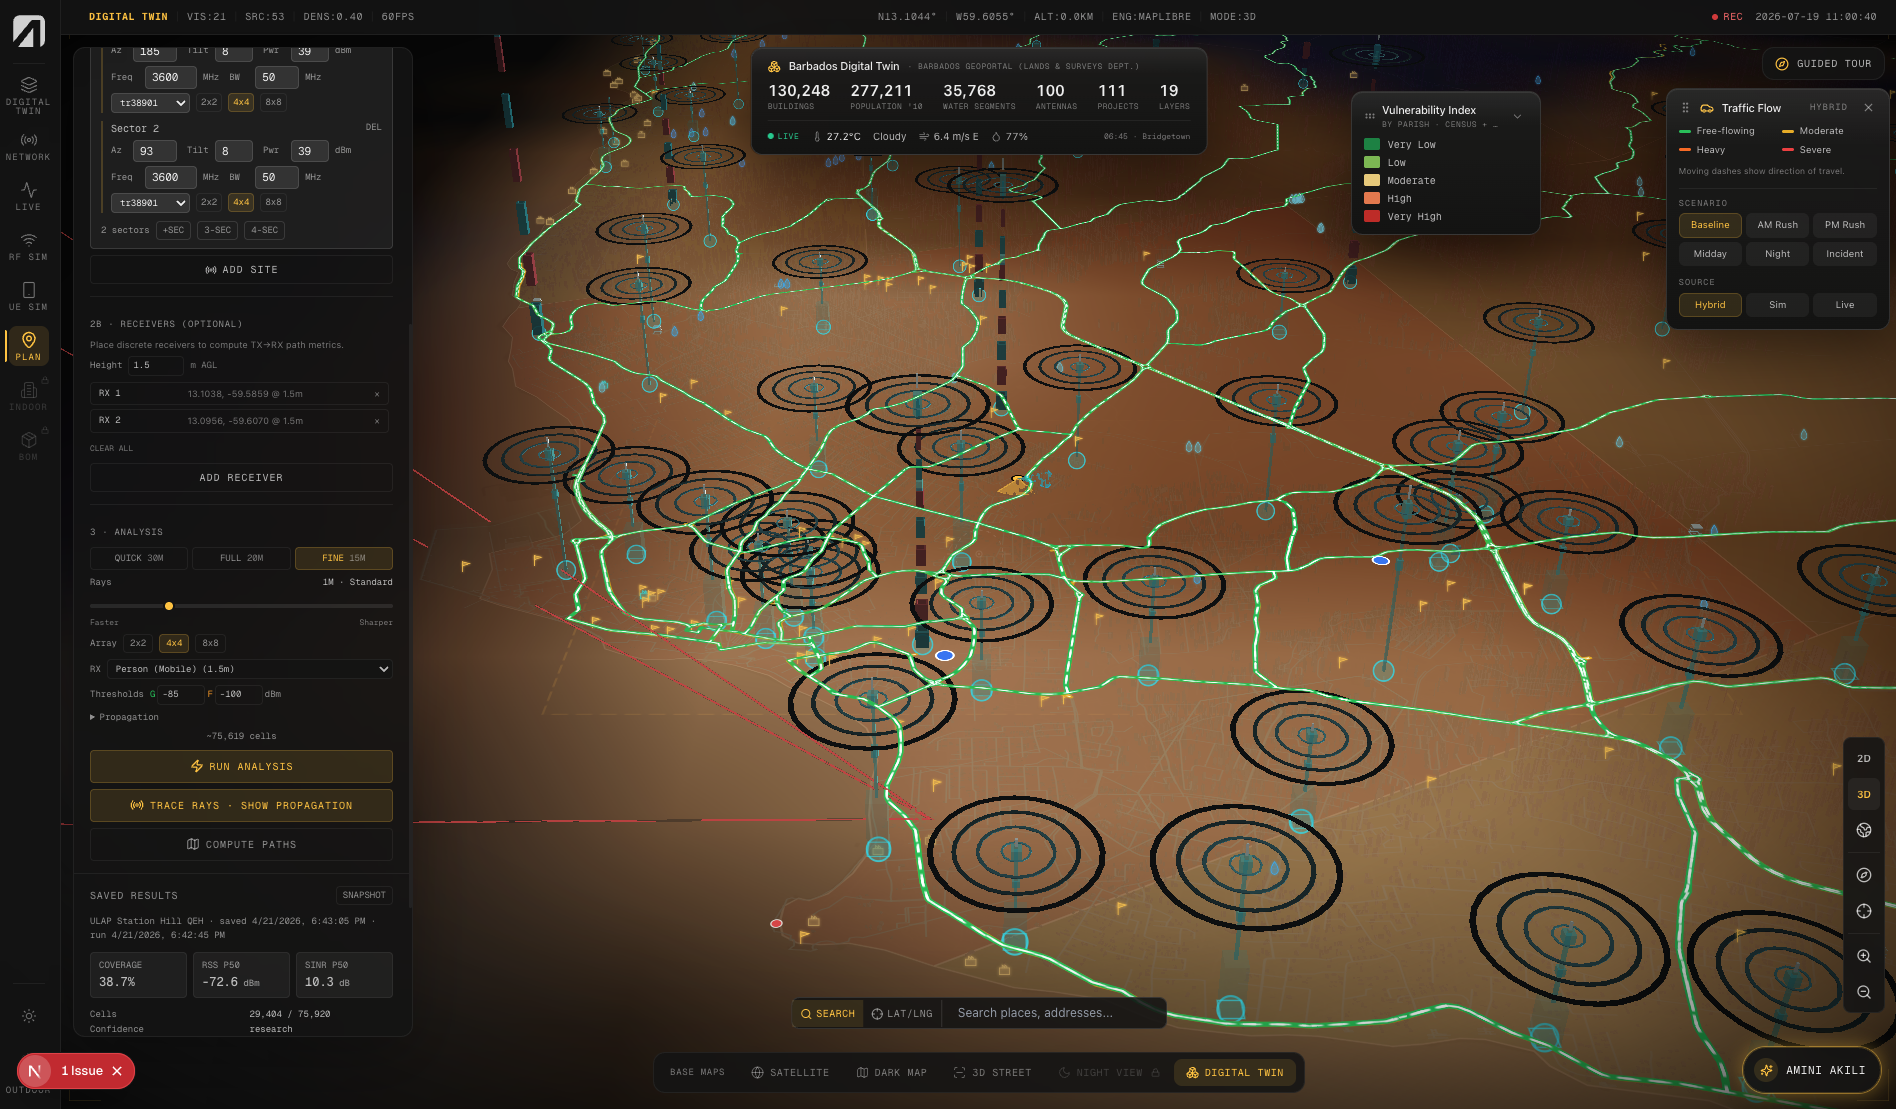
\includegraphics[width=\linewidth]{bbd-digital-twin-1.png}
\captionof{figure}{Network coverage planning in the twin's PLAN mode. Per-sector
RF configuration (azimuth, tilt, and power; 3600~MHz, 50~MHz bandwidth) is
propagated with a 3GPP TR~38.901 channel model over national infrastructure and
the parish-vulnerability surface. Discrete receivers yield per-run statistics:
38.7\% coverage, $-72.6$~dBm median RSS, and 10.3~dB median SINR across
$\sim$75{,}619 cells. Concentric rings are predicted per-site coverage cells---
the dual-function radio infrastructure repurposed for ISAC sensing in
\S\ref{sec:physical}.}
\label{fig:rf-coverage}
\end{minipage}\hfill
\begin{minipage}[t]{0.485\textwidth}
\centering
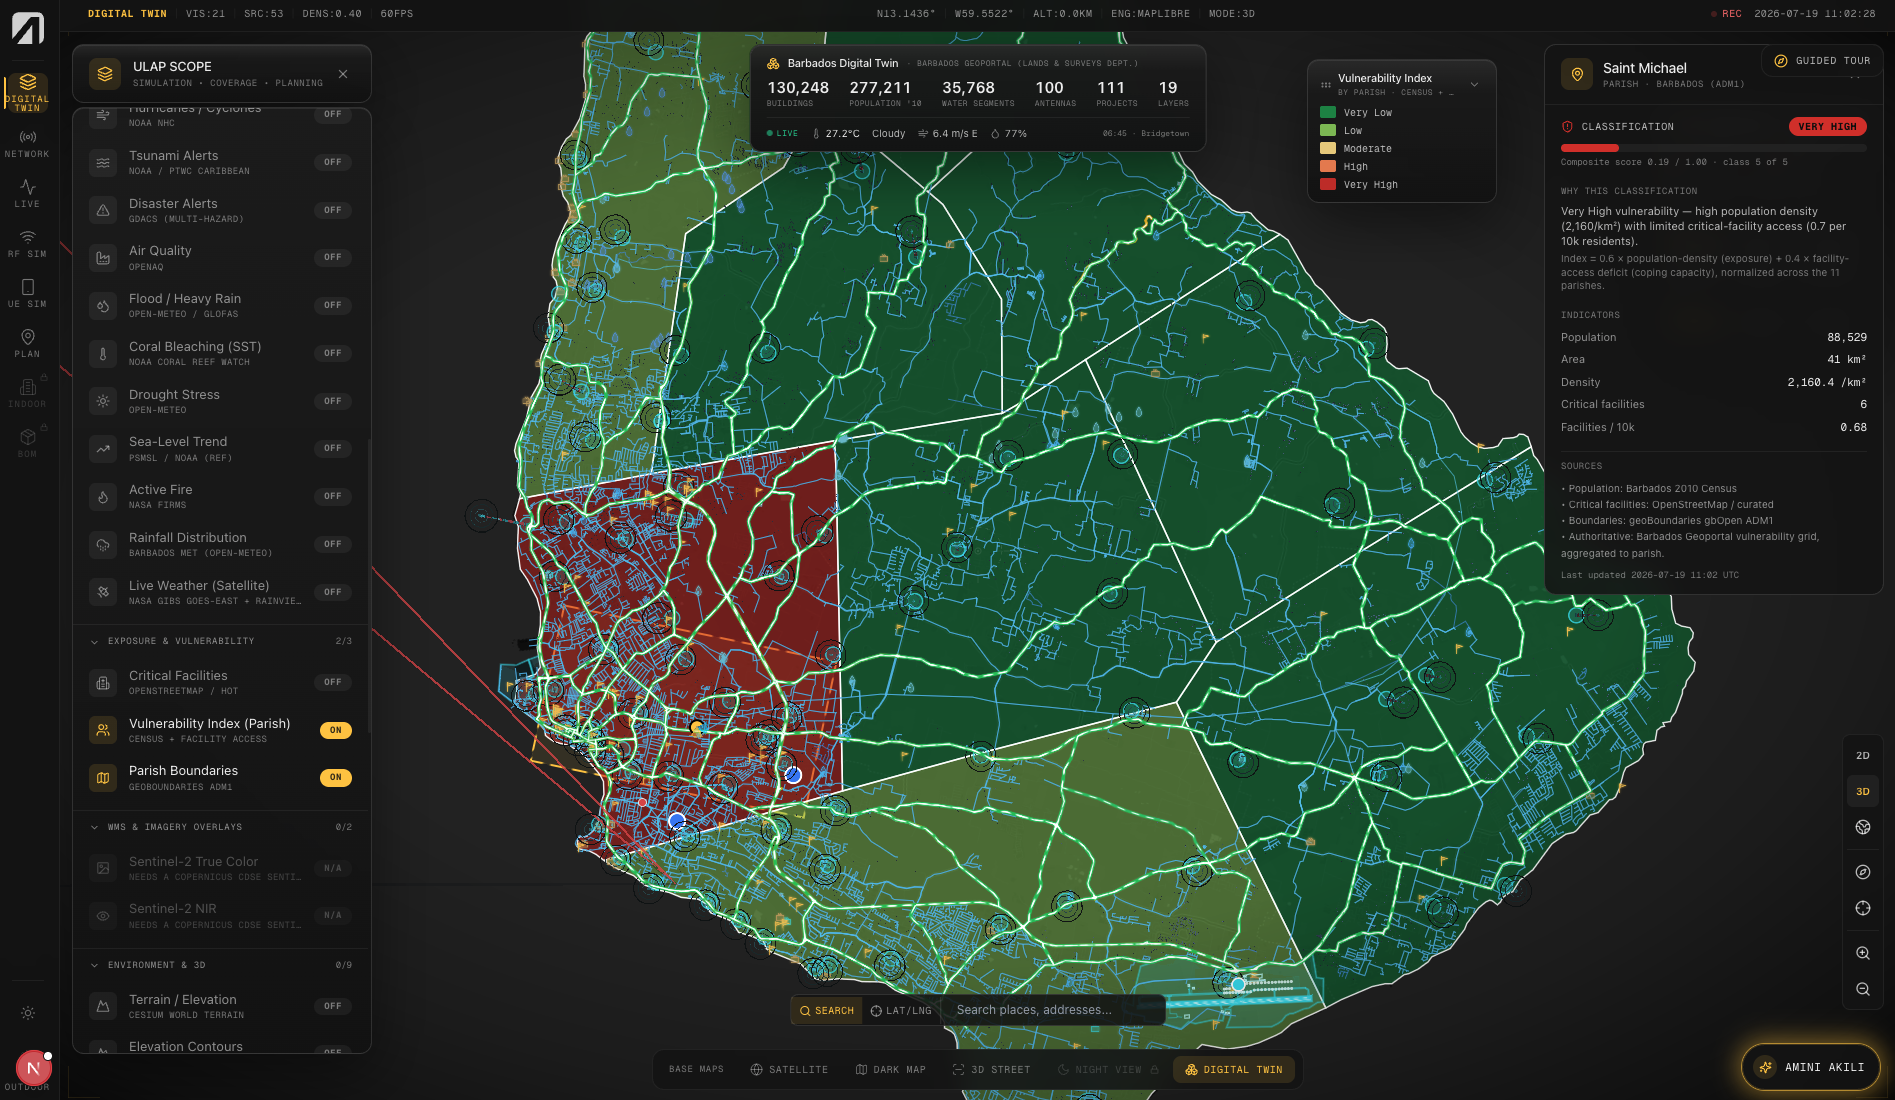
\includegraphics[width=\linewidth]{bbd-digital-twin-2.png}
\captionof{figure}{Authoritative per-parish vulnerability index. Parishes are
graded Very Low to Very High from the Barbados Geoportal vulnerability grid
aggregated to ADM1 boundaries. The inspected parish, Saint Michael, is Very High
(composite 0.19/1.00; class 5 of 5), reflecting population density
(2,160/km$^2$; population 88,529) and a critical-facility access deficit
(0.68 facilities per 10,000 residents). Its panel names the Barbados 2010
Census, OSM/curated critical facilities, geoBoundaries ADM1, and authoritative
Geoportal grid, realizing the labeled-provenance contract of
\S\ref{sec:impl-governance}.}
\label{fig:vulnerability-index}
\end{minipage}

\vspace{0.8em}
\begin{minipage}[t]{0.485\textwidth}
\centering
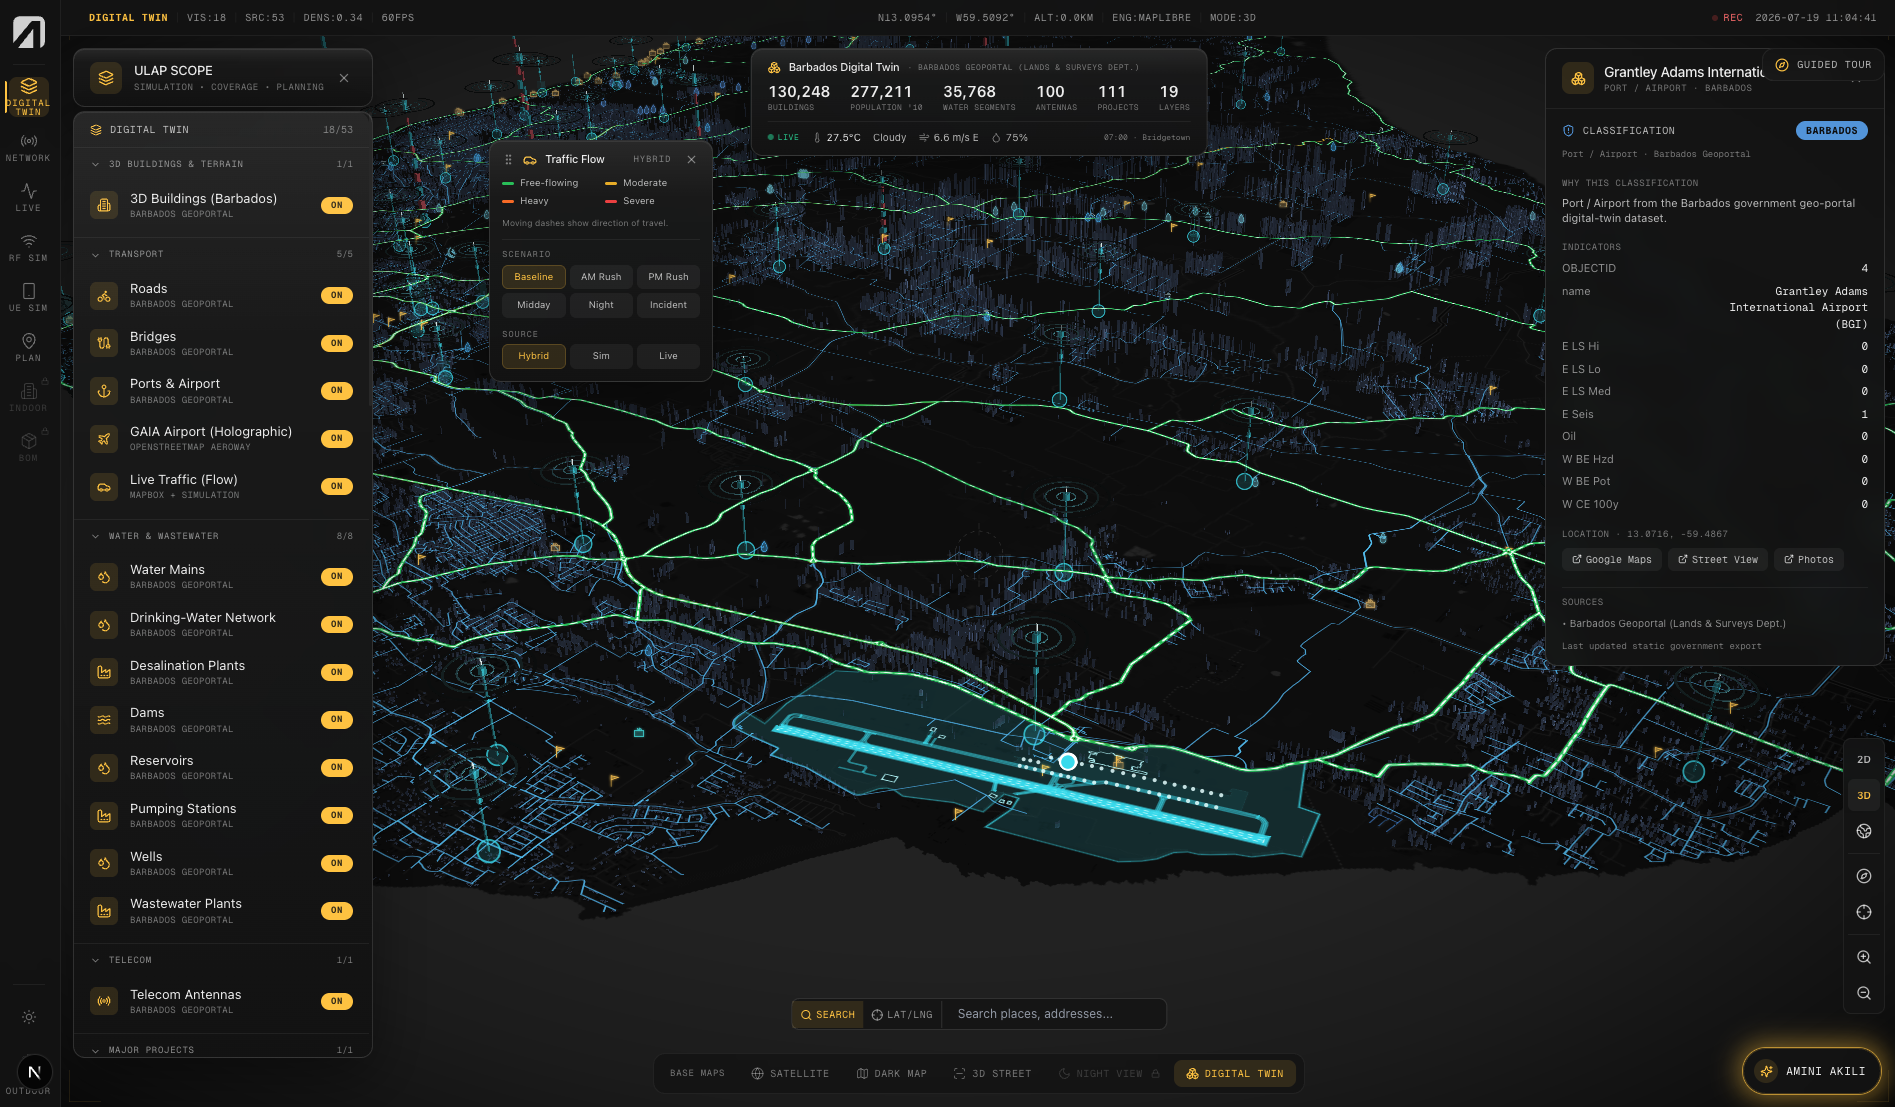
\includegraphics[width=\linewidth]{bbd-digital-twin-3.png}
\captionof{figure}{Government-asset inspection with hazard attributes. The
holographic 3D render selects Grantley Adams International Airport (BGI) on the
dark-map building and terrain base. Its inspect panel exposes provenance
(Barbados Geoportal) and per-asset hazard return-period fields---landslide
\texttt{E\_LS}, seismic \texttt{E\_Seis}, and coastal/rainfall flood
\texttt{W\_CE}/\texttt{W\_BE}---used to join critical assets to climate-risk
models (\S\ref{sec:impl-provenance}).}
\label{fig:airport-inspect}
\end{minipage}\hfill
\begin{minipage}[t]{0.485\textwidth}
\centering
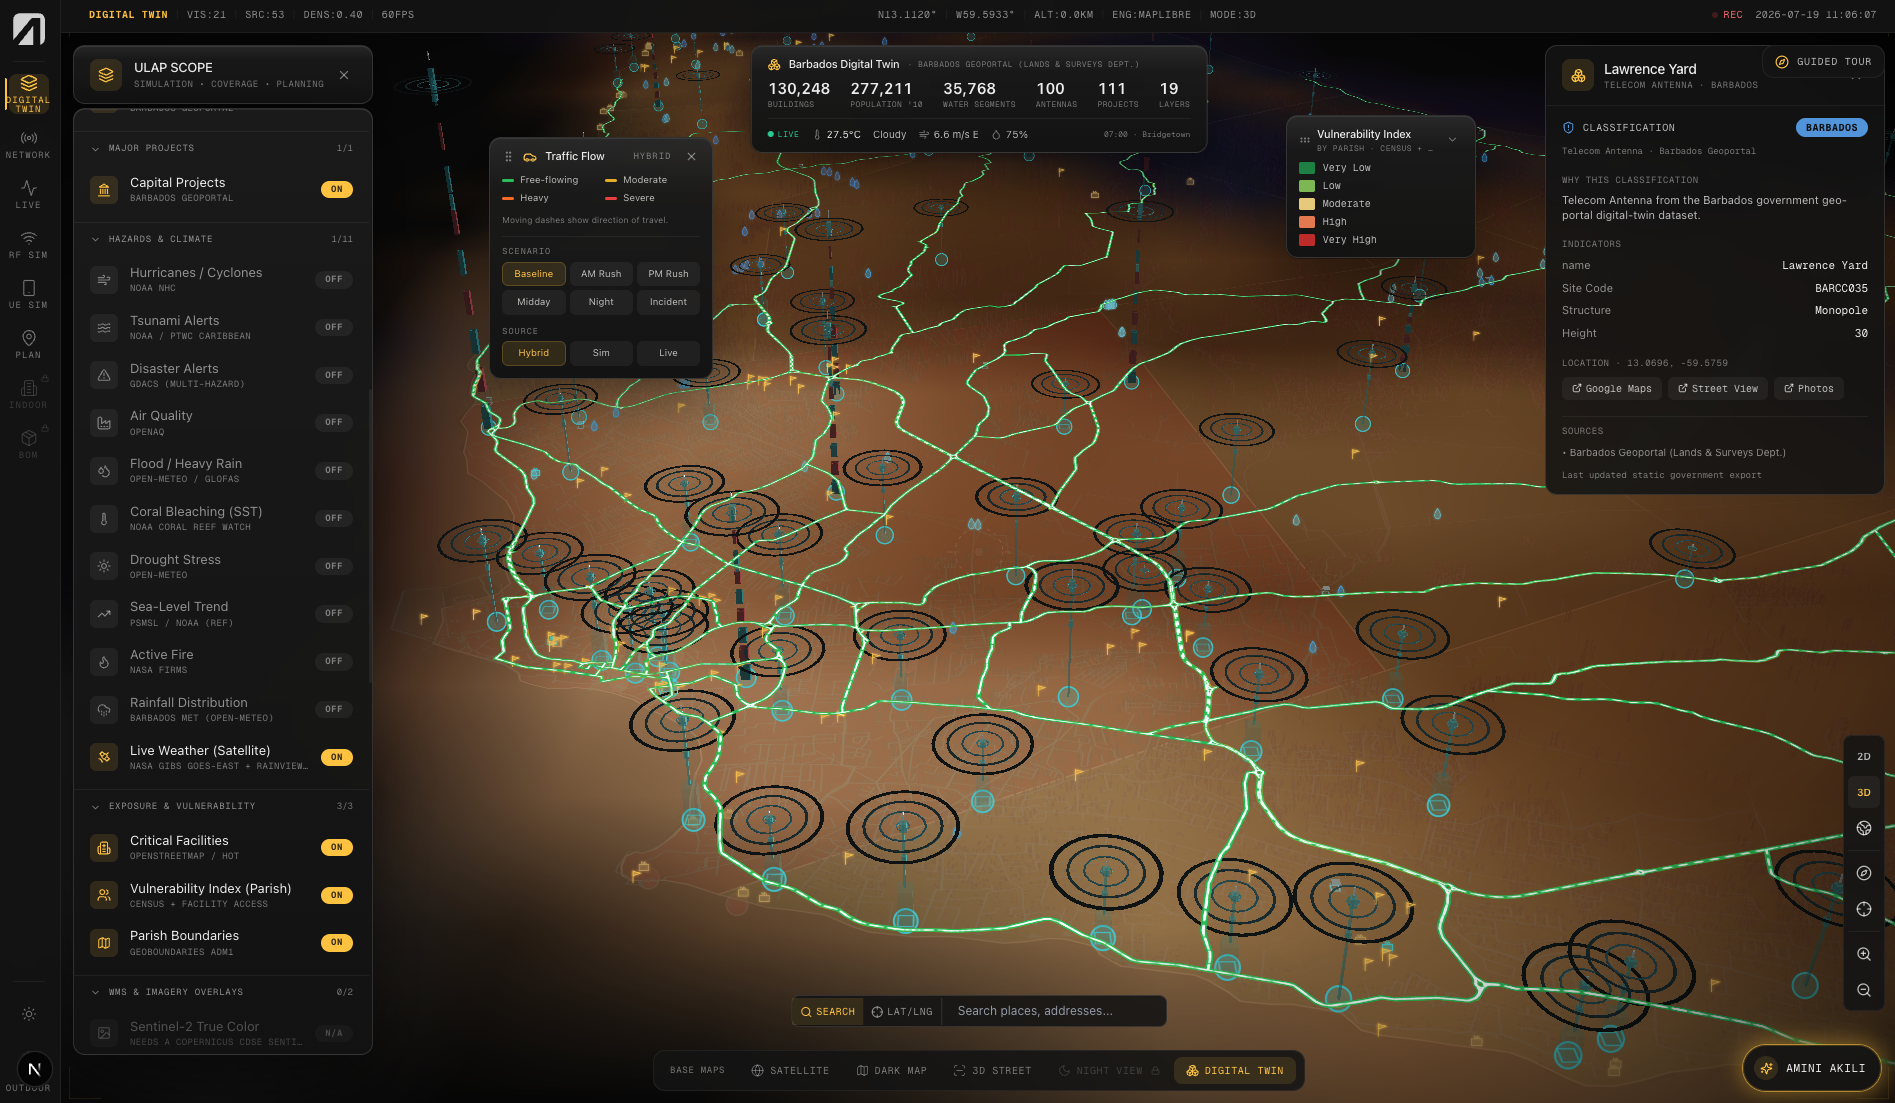
\includegraphics[width=\linewidth]{bbd-digital-twin-4.png}
\captionof{figure}{Telecom asset in its coverage-and-exposure context. A 30~m
monopole at Lawrence Yard (site \texttt{BARCC035}) is inspected over predicted RF
coverage cells and the parish-vulnerability surface, together with the live
weather/KPI header and traffic-flow scenario controls. This is the deployed
telecom layer that becomes the network-as-sensor substrate in the S-CDT.}
\label{fig:antenna-inspect}
\end{minipage}
\end{figure*}

\begin{figure*}[p]
\centering
\captionsetup{font=scriptsize,labelfont=bf,skip=3pt}
\begin{minipage}[t]{0.485\textwidth}
\centering
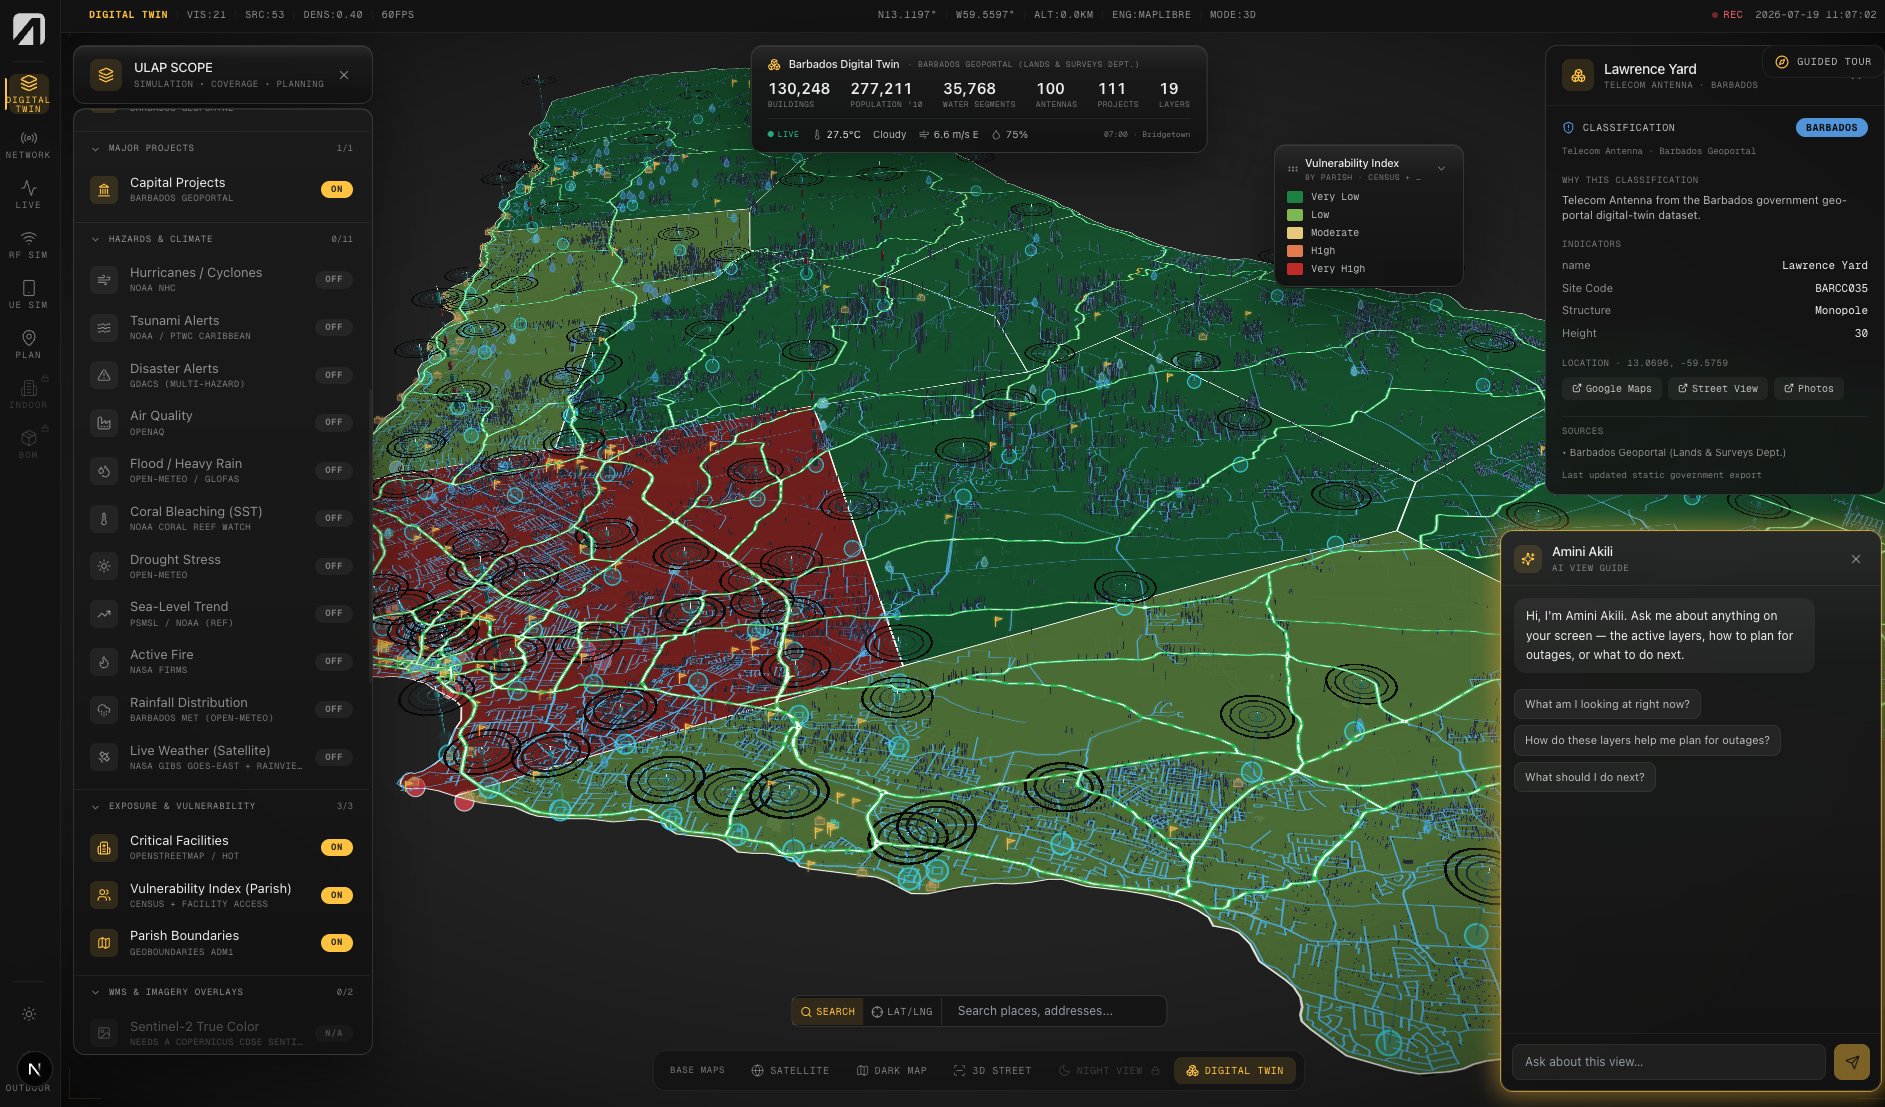
\includegraphics[width=\linewidth]{bbd-digital-twin-5.png}
\captionof{figure}{Natural-language interaction layer (Amini Akili). The in-map
generative assistant answers grounded questions about the current view,
including active layers, outage planning, and recommended next actions. Shown
over the parish-vulnerability choropleth with the Very High parish highlighted,
it realizes interaction layer~6 of Table~\ref{tab:map} and prefigures the GovChat
query surface in \S\ref{sec:roadmap}.}
\label{fig:akili-assistant}
\end{minipage}\hfill
\begin{minipage}[t]{0.485\textwidth}
\centering
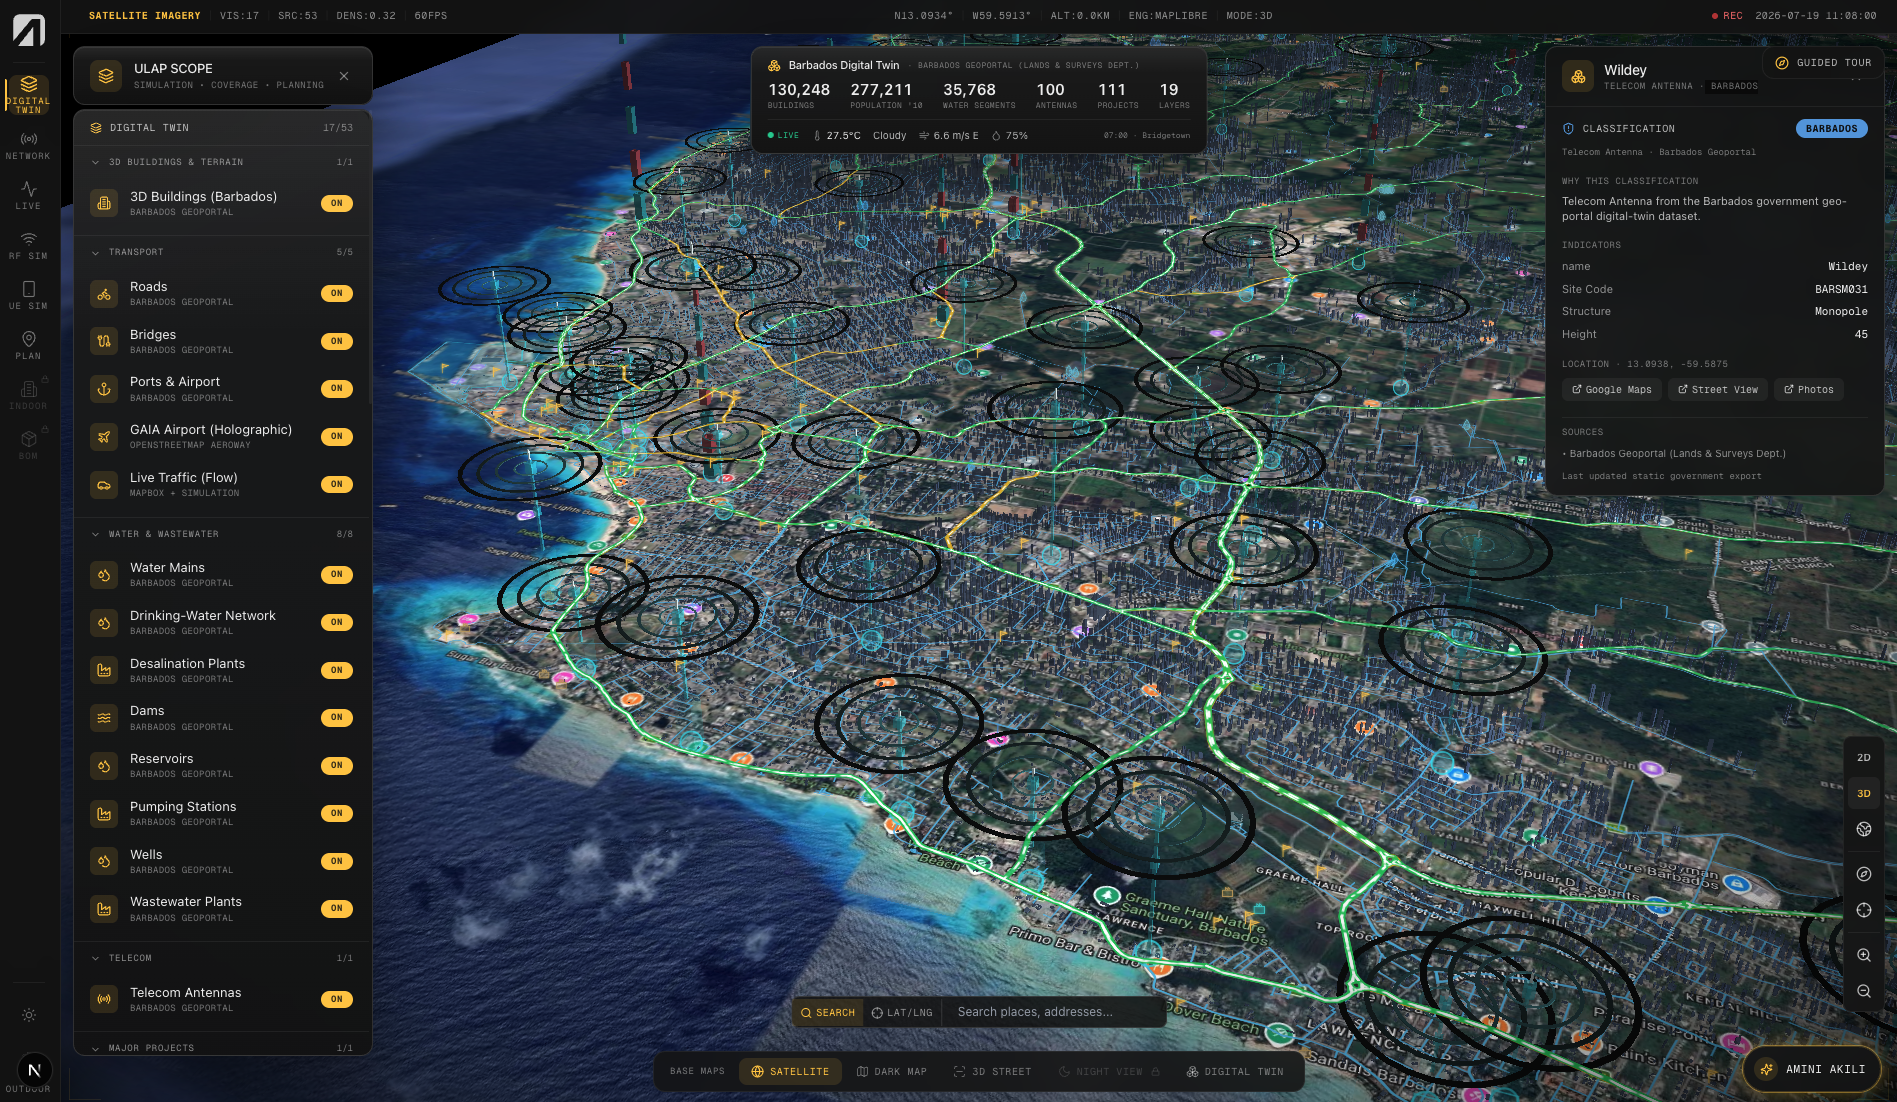
\includegraphics[width=\linewidth]{bbd-digital-twin-6.png}
\captionof{figure}{Twin over satellite imagery in oblique 3D. The Bridgetown and
south-coast conurbation combines the potable-water network (cyan), road network
(green), points of interest, and predicted antenna coverage cells on a satellite
basemap. Inspection of the 45~m Wildey monopole (site \texttt{BARSM031})
demonstrates multi-source fusion layered over the authoritative government
export.}
\label{fig:bridgetown-3d}
\end{minipage}

\vspace{0.8em}
\begin{minipage}[t]{0.64\textwidth}
\centering
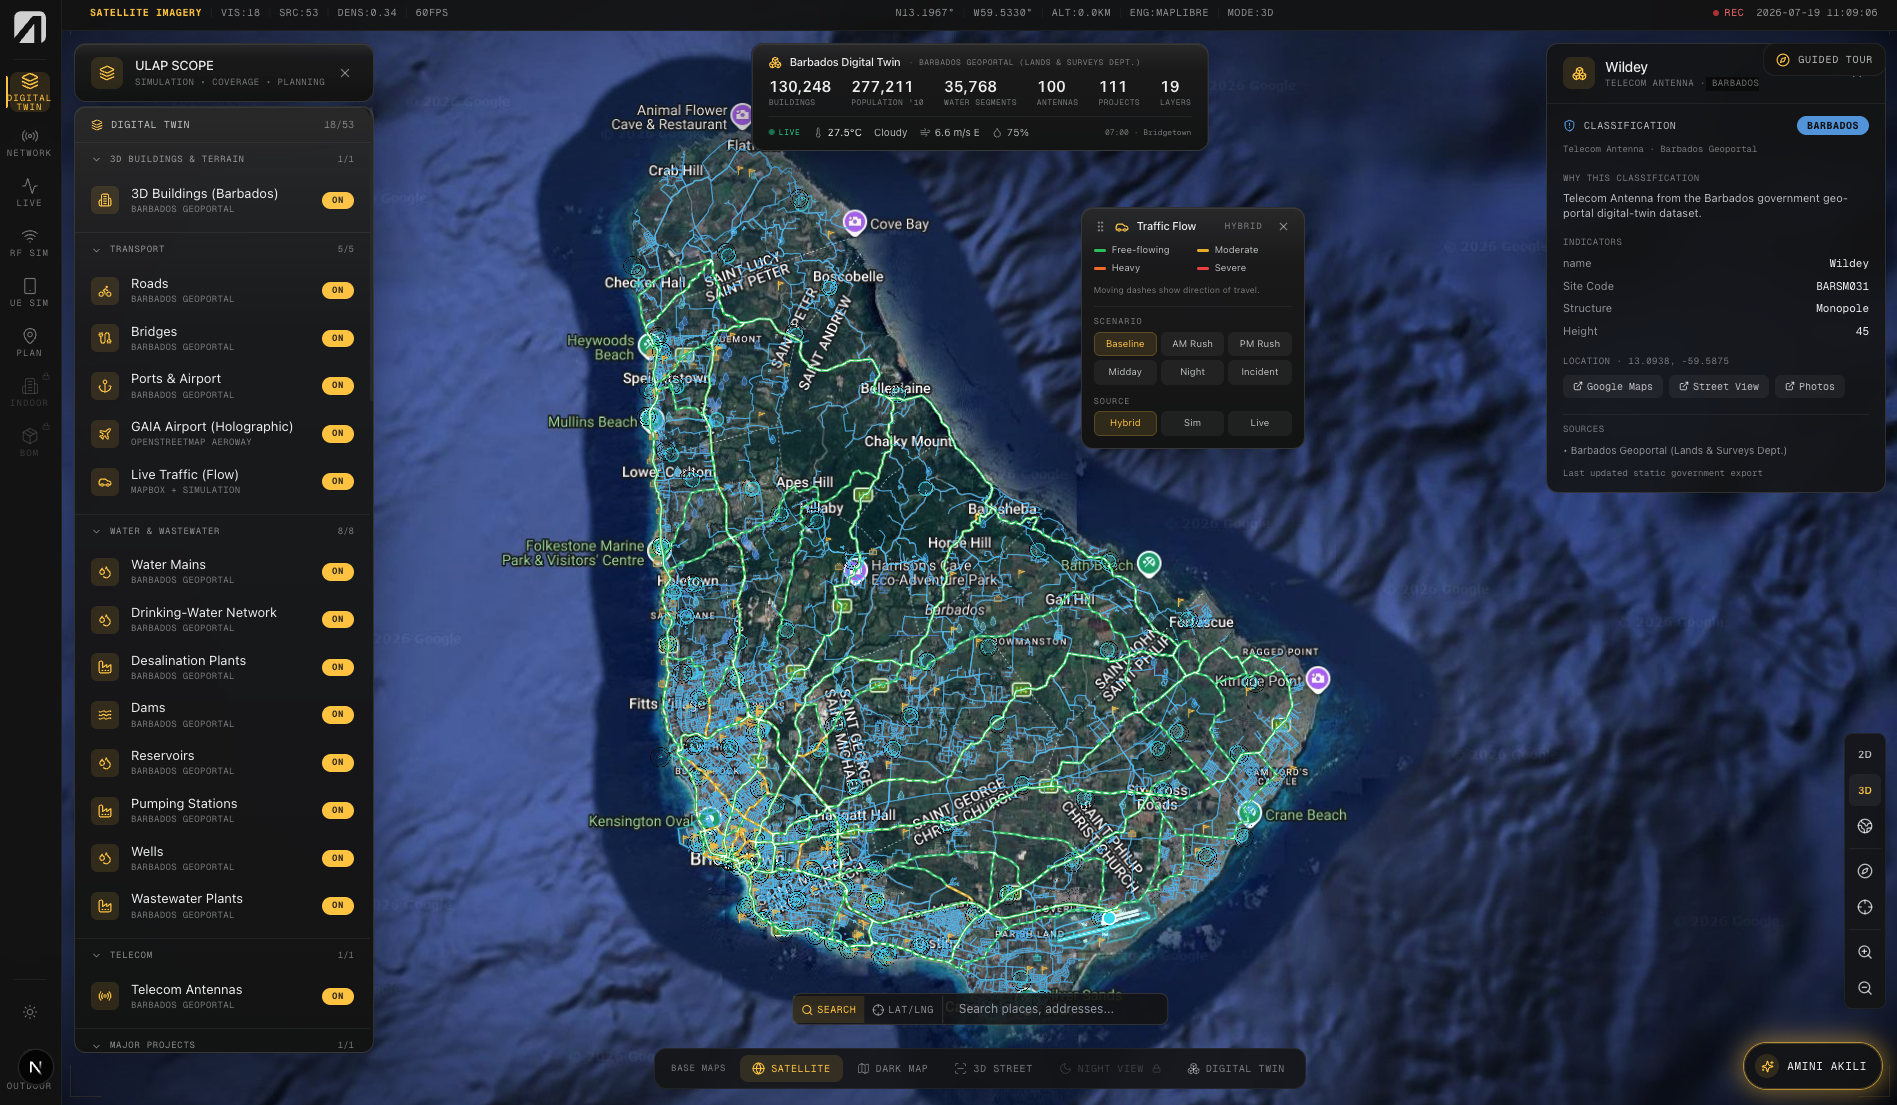
\includegraphics[width=\linewidth]{bbd-digital-twin-7.png}
\captionof{figure}{National context view. The full island of Barbados
(166~km$^2$) appears on a satellite basemap with complete road and water
networks, parish labels, traffic-flow scenario controls, and asset inspection.
This is the bounded, high-fidelity reference deployment generalized to the
Philippine archipelago in \S\ref{sec:deploy}.}
\label{fig:island-overview}
\end{minipage}
\end{figure*}
\clearpage

\section{Conclusion and Future Work}
We have argued that the cheapest path to national-scale climate perception for
island and archipelagic states is not more dedicated sensors but a
re-conception of the network itself as the nation's sensing nervous system,
orchestrated by a sovereign, cognitively closed-loop digital twin. The S-CDT
unifies the built-environment and earth-system digital-twin traditions,
grounds its perception in the emerging ETSI and 3GPP ISAC standards, controls
under realistic RAN delay via belief-state estimation, and treats sovereignty
and physical-layer privacy as primary. Future work includes: field
quantification of CSI-based rainfall accuracy against gauge networks in the
Caribbean band plan; sim-to-real transfer of the PPO orchestration policy on an
O-RAN testbed; formal verification of the minimized-kernel trust boundaries; and
a measurement study of the L1/L2/L3 privacy-waveform trade-off curve.

\balance
\begin{thebibliography}{99}
\small
\bibitem{undp_sids} UNDP Climate Promise, ``Small Island Developing States are on
the frontlines of climate change,'' 2023. [Online]. Available:
\url{https://climatepromise.undp.org/news-and-stories/small-island-developing-states-are-frontlines-climate-change-heres-why}

\bibitem{wef_barbados} World Economic Forum, ``Unpredictable weather events are
reshaping the future of small states and island nations, like Barbados,'' 2023.
[Online]. Available:
\url{https://www.weforum.org/stories/2023/06/barbados-climate-resilience-data-technology/}

\bibitem{ndtp} Centre for Digital Built Britain, ``National Digital Twin
Programme.'' [Online]. Available:
\url{https://www.cdbb.cam.ac.uk/what-we-did/national-digital-twin-programme}

\bibitem{gemini} Centre for Digital Built Britain, ``The Gemini Principles,''
2018. [Online]. Available:
\url{https://www.cdbb.cam.ac.uk/system/files/documents/TheGeminiPrinciples.pdf}

\bibitem{vsg} Government Technology Agency of Singapore (GovTech), ``5 things to
know about Virtual Singapore.'' [Online]. Available:
\url{https://www.tech.gov.sg/technews/5-things-to-know-about-virtual-singapore/}

\bibitem{destine} European Commission, ``Destination Earth (DestinE).''
[Online]. Available:
\url{https://digital-strategy.ec.europa.eu/en/policies/destination-earth}

\bibitem{ericsson_isac} Ericsson, ``Integrated Sensing and Communication
(ISAC) explained.'' [Online]. Available:
\url{https://www.ericsson.com/en/6g/isac}

\bibitem{ericsson_isc001} Ericsson Technology Review, ``Sensing in 6G: use cases
and architecture.'' [Online]. Available:
\url{https://www.ericsson.com/en/reports-and-papers/ericsson-technology-review/articles/sensing-in-6g-use-cases-and-architecture}

\bibitem{etsi_isc001} ETSI, ``ETSI publishes first Report on ISAC Use Cases for
6G'' (GR ISC~001), April 2025. [Online]. Available:
\url{https://www.etsi.org/newsroom/press-releases/2520-etsi-publishes-first-report-on-isac-use-cases-for-6g/}

\bibitem{etsi_isc003} ETSI, ``New Report on ISAC System and RAN Architectures''
(GR ISC~003), 2026. [Online]. Available:
\url{https://www.etsi.org/newsroom/news/2646-gr-isc-003-6g-isac-system-ran-architectures/}

\bibitem{tr22837} 3GPP, ``TR 22.837: Feasibility Study on Integrated Sensing and
Communication,'' Release~19.

\bibitem{tr38901} 3GPP, ``TR 38.901: Study on channel model for frequencies from
0.5 to 100 GHz'' (ISAC extensions), Release~19.

\bibitem{rel19survey} ``A Comprehensive Survey of 3GPP Release~19 ISAC Channel
Modeling,'' arXiv:2512.03506, 2025. [Online]. Available:
\url{https://arxiv.org/abs/2512.03506}

\bibitem{itur838} ITU-R, ``Recommendation P.838: Specific attenuation model for
rain for use in prediction methods.''

\bibitem{raingauge} ``RainGaugeNet: CSI-Based Sub-6 GHz Rainfall Attenuation
Measurement and Classification for ISAC Applications,'' arXiv:2501.02175, 2025.
[Online]. Available: \url{https://arxiv.org/abs/2501.02175}

\bibitem{oran_isac} ``Toward Native ISAC Support in O-RAN Architectures for
6G,'' arXiv:2603.03607, 2026. [Online]. Available:
\url{https://arxiv.org/abs/2603.03607}

\bibitem{oppo_kernel} OPPO, ``A Versatile 6G with Minimized Kernel'' (6G White
Paper). [Online]. Available:
\url{https://www.oppo.com/content/dam/oppo/common/mkt/footer/OPPO-6G-White-Paper-EN.pdf}

\bibitem{oppo_sec} OPPO, ``6G Security Architecture: Intelligent Security Built
on Zero Trust'' (6G Security White Paper). [Online]. Available:
\url{https://www.oppo.com/content/dam/oppo/common/mkt/footer/OPPO-6G-Security-WhitePaper-EN.pdf}

\bibitem{bbdgeo} Government of Barbados, ``Barbados Geoportal --- Lands \& Surveys
Department.'' [Online]. Available: \url{https://geoportal-bds-lsdept.hub.arcgis.com/}
\end{thebibliography}

\end{document}
